\documentclass[12pt]{report}
\date{June 19, 2017}
\usepackage[utf8]{inputenc}
\usepackage{fullpage}
\usepackage{graphicx}


\begin{document}
	\title{Multi-agent transport simulation. Hausaufgabe 1.}
	
\author{Timofey Volotskiy. Matrikelnr. 357563}
\maketitle

\section{Aufgabe 1 - Maßnahmen}

Für die Hausaufgabe wurde eine Tempo-30 Zone-Einführung in Berlin-Mitte ausgewählt. Ein Gebiet, wo alle Hauptstraßen eine zugelassene Geschwindigkeit von 30 km/h haben, ist von der Straßen begrenzt: 

\begin{itemize}
	\item Gitschiner Str. 
	\item Skalitzer Str. 
	\item Oberbaumbrücke 
	\item	Warschauer Str.
	\item	Petersburger Str.
	\item Danziger Str.
	\item Bernauer Str.
	\item Friedrichstraße
	\item Reinhardtstraße
	\item Ebertstraße
	\item Stresemannstraße
\end{itemize}


\section{Aufgabe 2 - Maßnahmen}

Um die obengenannte Maßnahme in der Simulation zu implementieren wurde das Netzwerk in einem JOSM Plugin modifiziert. Der Parameter $ "matsim:freespeed" $ wurde auf $ 8.(333) $ gesetzt.

\begin{center}
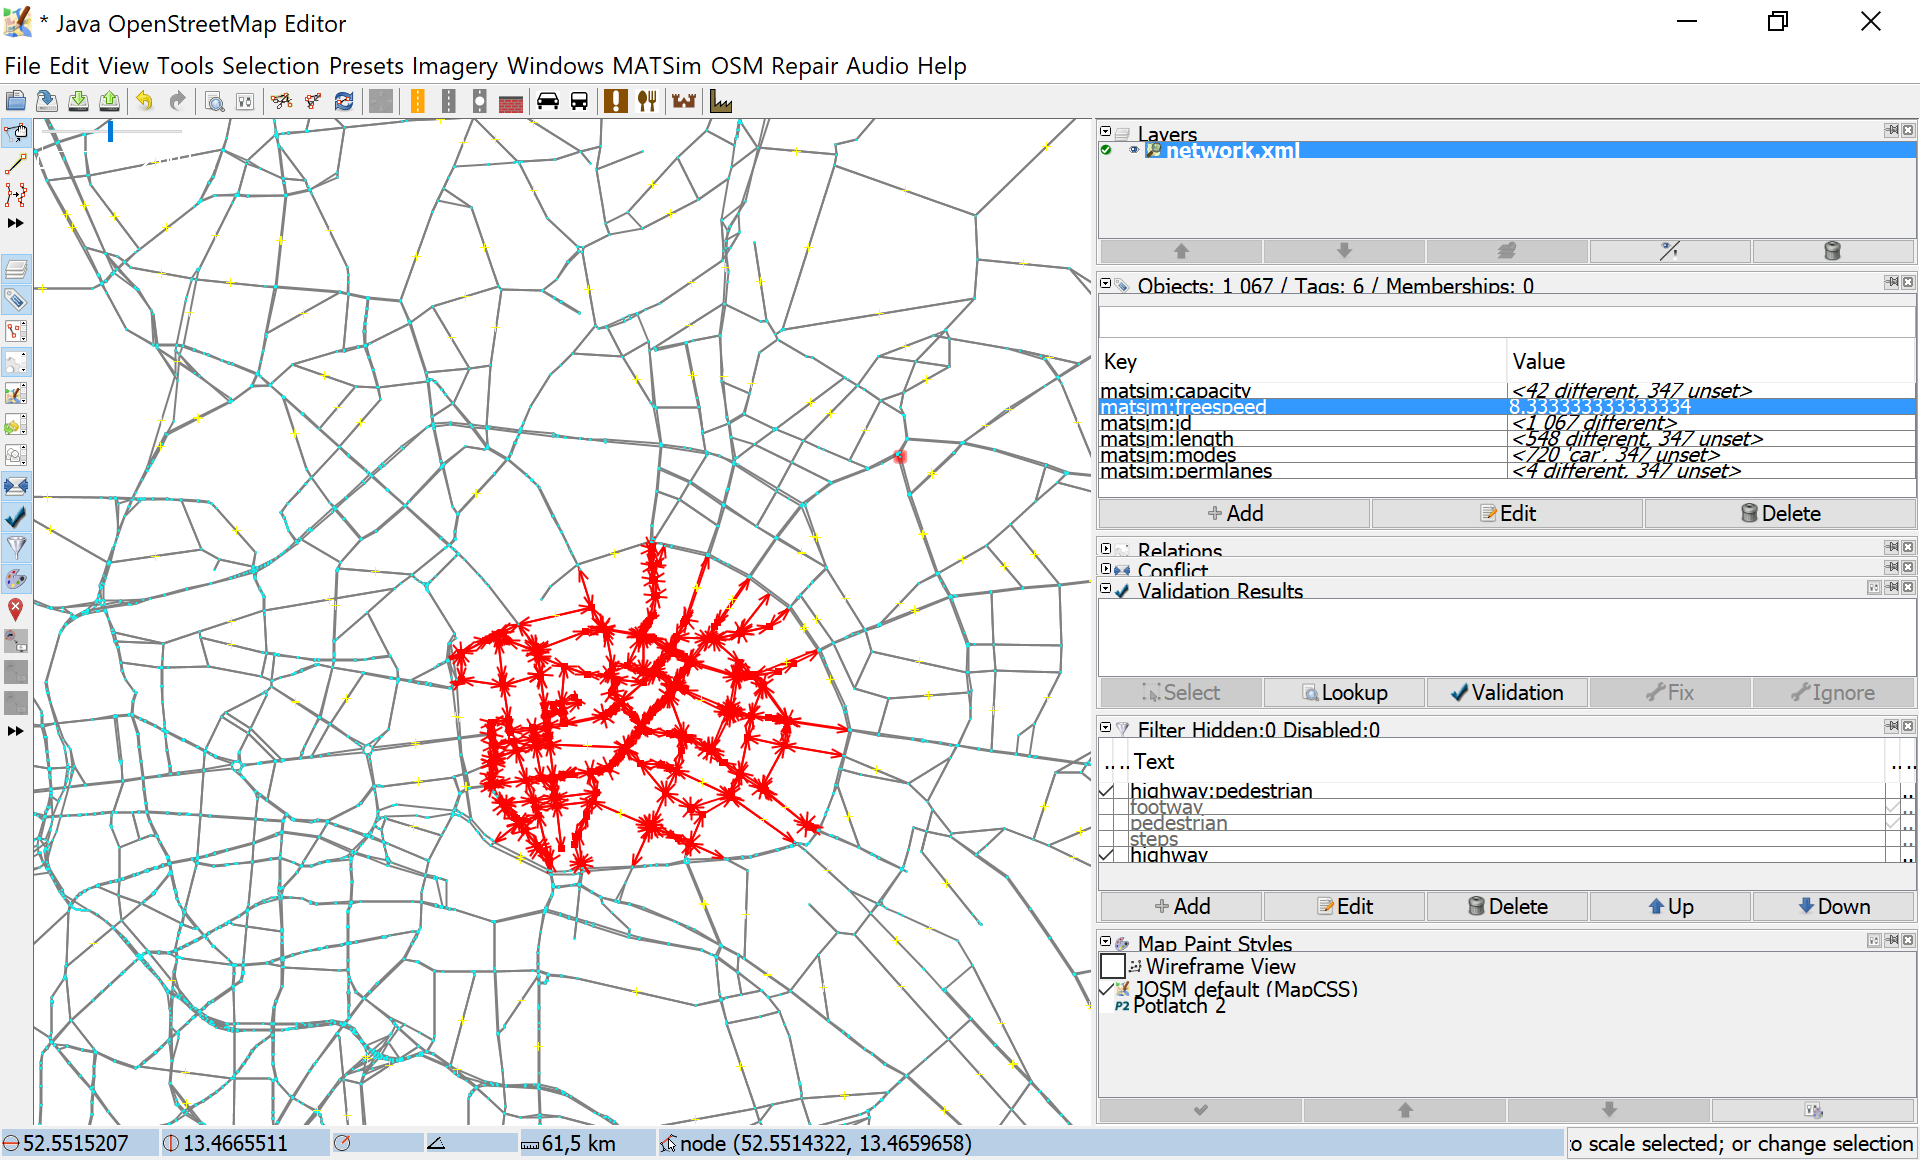
\includegraphics[width = 500]{tempo30zoneJOSM}
\end{center}


% Table generated by Excel2LaTeX from sheet 'accessibilities'
\begin{table}[htbp]
\centering
\caption{Table1}
\begin{tabular}{cc|c|c|c}
xcoord & ycoord & pt\_accessibility & population\_density & population\_density \\
950.0 & 950.0 & -3.7571823924145833 & 0.0   & 0.0 \\
1050.0 & 950.0 & -3.7571823924145833 & 0.0   & 0.0 \\
1150.0 & 950.0 & -3.882578022405829 & 0.0   & 0.0 \\
1250.0 & 950.0 & -4.021508262519376 & 0.0   & 0.0 \\
1350.0 & 950.0 & -4.162971175147671 & 0.0   & 0.0 \\
1450.0 & 950.0 & -4.836714194230462 & 0.0   & 0.0 \\
1550.0 & 950.0 & -4.979463123938224 & 0.0   & 0.0 \\
1650.0 & 950.0 & -5.1224321274009235 & 0.0   & 0.0 \\
1750.0 & 950.0 & -5.265533679137514 & 0.0   & 0.0 \\
1850.0 & 950.0 & -5.940121198304677 & 0.0   & 0.0 \\
1950.0 & 950.0 & -6.083367628083968 & 0.0   & 0.0 \\
2050.0 & 950.0 & -6.2266561819814985 & 0.0   & 0.0 \\
2150.0 & 950.0 & -6.369975895236712 & 0.0   & 0.0 \\
2250.0 & 950.0 & -7.044719303317949 & 0.0   & 0.0 \\
2350.0 & 950.0 & -7.18808114889281 & 0.0   & 0.0 \\
2450.0 & 950.0 & -7.331457622397679 & 0.0   & 0.0 \\
2550.0 & 950.0 & -7.157324534961399 & 0.0   & 0.0 \\
2650.0 & 950.0 & -7.01424905807054 & 0.0   & 0.0 \\
2750.0 & 950.0 & -6.871238687761487 & 0.0   & 0.0 \\
2850.0 & 950.0 & -6.728311051145136 & 0.0   & 0.0 \\
2950.0 & 950.0 & -6.054090752342283 & 0.0   & 0.0 \\
3050.0 & 950.0 & -5.9114131917296096 & 0.0   & 0.0 \\
3150.0 & 950.0 & -5.768931191364208 & 0.0   & 0.0 \\
3250.0 & 950.0 & -5.626727153564026 & 0.0   & 0.0 \\
3350.0 & 950.0 & -4.953536971428138 & 0.0   & 0.0 \\
3450.0 & 950.0 & -4.812401328307441 & 0.0   & 0.0 \\
3550.0 & 950.0 & -4.672388914627426 & 0.0   & 0.0 \\
3650.0 & 950.0 & -4.534540848080349 & 0.0   & 0.0 \\
3750.0 & 950.0 & -3.8702593973272506 & 0.0   & 0.0 \\
3850.0 & 950.0 & -3.752349588097854 & 0.0   & 0.0 \\
3950.0 & 950.0 & -3.6929231967313116 & 0.0   & 0.0 \\
4050.0 & 950.0 & -3.752349588097854 & 0.0   & 0.0 \\
950.0 & 1050.0 & -3.7571823924145833 & 0.0   & 0.0 \\
1050.0 & 1050.0 & -3.7571823924145833 & 73.0  & 73.0 \\
1150.0 & 1050.0 & -3.882578022405829 & 0.0   & 0.0 \\
1250.0 & 1050.0 & -4.021508262519376 & 0.0   & 0.0 \\
1350.0 & 1050.0 & -4.162971175147671 & 0.0   & 0.0 \\
1450.0 & 1050.0 & -4.836714194230462 & 0.0   & 0.0 \\
1550.0 & 1050.0 & -4.979463123938224 & 0.0   & 0.0 \\
1650.0 & 1050.0 & -5.1224321274009235 & 0.0   & 0.0 \\
1750.0 & 1050.0 & -5.265533679137514 & 0.0   & 0.0 \\
1850.0 & 1050.0 & -5.940121198304677 & 0.0   & 0.0 \\
1950.0 & 1050.0 & -6.083367628083968 & 0.0   & 0.0 \\
2050.0 & 1050.0 & -6.2266561819814985 & 0.0   & 0.0 \\


\end{tabular}%
\label{tab:addlabel}%
\end{table}%







 \end{document}